\chapter{Analisis}
\label{chap:analisis}

Pada bab ini akan dibahas analisis terhadap teori-teori yang telah dibahas sebelumnya. Analisis akan meliputi studi kasus untuk penerapan metode \textit{secret sharing} Shamir, pemilihan \begin{math}n\end{math} dan \begin{math}k\end{math}, analisis proses, dan perancangan diagram.

\section{Studi Kasus}

Pada bagian ini akan dibahas studi kasus tentang bagaimana penerapan metode \textit{secret sharing} Shamir untuk banyak \textit{password}. Studi kasus meliputi pengenalan kasus, proses penyimpanan \textit{password}, dan proses rekonstruksi \textit{password}.

\subsection{Pengenalan Kasus}\label{subsec:pengenalankasus}

Langkah awal yang dibutuhkan untuk mengembalikan banyak \textit{password} dengan metode \textit{secret sharing} Shamir, diperlukan beberapa tahap proses. Proses pertama adalah proses penyimpanan \textit{password}. Kemudian, proses selanjutnya adalah proses untuk mengembalikan banyak \textit{password}. Proses pertama membutuhkan beberapa \textit{password}. Untuk \begin{math}n\end{math} buah \textit{password}, maka akan dibuat \begin{math}n\end{math} buah pertanyaan keamanan. Sementara itu, untuk proses mengembalikan \textit{password} dibutuhkan pertanyaan keamanan yang sudah dibuat dalam proses sebelumnya.

Untuk kedua proses di atas, diasumsikan banyak \textit{password} yang akan disimpan sebanyak 5 buah. Setiap \textit{password} akan diberi label \begin{math}p_1\end{math}, \begin{math}p_2\end{math}, sampai \begin{math}p_5\end{math}. Persamaan \ref{eq:passwords1} sampai \ref{eq:passwords5} menunjukkan \begin{math}p_1\end{math} sampai \begin{math}p_5\end{math}.

\begin{gather}
	p_1 = 123456 \label{eq:passwords1} \\
	p_2 = password \label{eq:passwords2} \\
	p_3 = hello123 \label{eq:passwords3} \\
	p_4 = secret \label{eq:passwords4} \\
	p_5 = foobar \label{eq:passwords5}
\end{gather}

\subsection{Proses Penyimpanan \textit{Password}}\label{subsec:simpanpassword}

Proses penyimpanan \textit{password} dibagi menjadi 2 proses, yaitu proses pembangunan \textit{share} untuk masing-masing \textit{password} dan proses enkripsi dari setiap \textit{share} yang sudah dibangun. Pada bagian ini akan dibahas kedua proses tersebut.

\subsubsection{Proses Pembangunan \textit{Share}}

Pada proses ini, akan dilakukan pembangunan \textit{share} dari masing-masing \textit{password}. Langkah-langkah untuk membangun share adalah sebagai berikut.

\begin{enumerate}
	\item Membagi setiap \textit{password} \begin{math}p_i\end{math} menjadi beberapa karakter, masing-masing karakter akan diubah menjadi nilai ASCIInya, \begin{math}c_1, c_2, ..., c_m\end{math}.
		\item Memilih nilai \begin{math}n\end{math}, yaitu banyak \textit{share} yang akan dibangun.
	\item Memilih nilai \begin{math}k\end{math}, yaitu banyak minimal pertanyaan keamanan yang harus dijawab dengan benar, dimana \begin{math}0 < k \leq n\end{math}.
	\item Memilih \begin{math}k-1\end{math} angka acak, \begin{math}d_1, d_2, ..., d_{k-1}\end{math}, untuk masing-masing karakter \begin{math}c_1, c_2, ..., c_m\end{math}.
	\item Membentuk fungsi \begin{math}f_m(x)\end{math} untuk masing-masing karakter \begin{math}c_1, c_2, ..., c_m\end{math}. 
	Komponen dari fungsi \begin{math}f_m(x)\end{math} terdiri atas \begin{math}c_m\end{math} sebagai konstanta tanpa koefesien, \begin{math}d_1, d_2, ..., d_{k-1}\end{math} sebagai konstanta dengan koefesien. Persamaan \ref{eq:fungsifx} menunjukkan persamaan dari fungsi \begin{math}f_m(x)\end{math} yang harus dibentuk.
	\begin{equation}
		f_m(x) = c_m + d_1x + d_2x^2 + d_3x^3 + ... + d_{k-1}x^{k-1}
		\label{eq:fungsifx}
	\end{equation}
	\item Menghitung masing-masing nilai \begin{math}x\end{math} dari \begin{math}x=1, x=2, ..., x=n\end{math} untuk fungsi \begin{math}f_m(x)\end{math}.
	\item Nilai \begin{math}f_m(1)\end{math} sampai \begin{math}f_m(n)\end{math} adalah nilai \textit{share} untuk password \begin{math}p_i\end{math}.
\end{enumerate}

Kembali kepada kasus pada Subbab \ref{subsec:pengenalankasus}, misalkan \textit{password} yang akan dibangun \textit{share-share}nya adalah \begin{math}p_1\end{math}. Langkah pertama adalah membagi \begin{math}p_1\end{math} menjadi beberapa karakter dan mengubah masing-masing karakter menjadi nilai ASCIInya. Persamaan \ref{eq:ubahascii1} sampai \ref{eq:ubahascii7} menunjukkan langkah pertama.

\begin{gather}
	p_1 = 123456 \label{eq:ubahascii1} \\
	c_1 = '1' = 49 \label{eq:ubahascii2} \\
	c_2 = '2' = 50 \label{eq:ubahascii3} \\
	c_3 = '3' = 51 \label{eq:ubahascii4} \\
	c_4 = '4' = 52 \label{eq:ubahascii5} \\
	c_5 = '5' = 53 \label{eq:ubahascii6} \\
	c_6 = '6' = 54 \label{eq:ubahascii7}
\end{gather}

Langkah selanjutnya adalah memilih nilai \begin{math}n\end{math}. Karena banyak \textit{password} \begin{math}p_i\end{math} adalah 5, maka banyak \textit{share} untuk masing-masing \textit{password} sebanyak 5. Maka, \begin{math}n=5\end{math}.

Setelah memilih nilai \begin{math}n\end{math}, langkah berikutnya adalah memilih nilai \begin{math}k\end{math}. Nilai \begin{math}k\end{math} ini nanti akan berhubungan dengan banyak minimal pertanyaan keamanan yang harus dijawab benar untuk mengembalikan \textit{password}. Untuk kasus ini, dipilih \begin{math}k=3\end{math}.

Langkah selanjutnya adalah memilih \begin{math}k-1\end{math} angka acak untuk masing-masing karakter \begin{math}c_1\end{math} sampai \begin{math}c_6\end{math}. Karena \begin{math}k=3\end{math}, maka dipilih 2 angka acak untuk masing-masing karakter. Berikut angka acak untuk masing-masing karakter.

\begin{itemize}
	\item \begin{math}c_1\end{math}: 12 dan 6.
	\item \begin{math}c_2\end{math}: 15 dan 11.
	\item \begin{math}c_3\end{math}: 22 dan 1.
	\item \begin{math}c_4\end{math}: 21 dan 3.
	\item \begin{math}c_5\end{math}: 19 dan 8.
	\item \begin{math}c_6\end{math}: 25 dan 17.
\end{itemize}

Setelah memilih angka acak untuk masing-masing karakter, langkah selanjutnya adalah membentuk fungsi \begin{math}f(x)\end{math} untuk masing-masing karakter. Maka, fungsi \begin{math}f_1(x)\end{math} sampai \begin{math}f_6(x)\end{math} yang dibentuk adalah sebagai ditunjukkan pada persamaan \ref{eq:fungsi1} sampai \ref{eq:fungsi6}.

\begin{gather}
	f_1(x) = 49 + 12x + 6x^2 \label{eq:fungsi1} \\
	f_2(x) = 50 + 15x + 11x^2 \label{eq:fungsi2} \\
	f_3(x) = 51 + 22x + x^2 \label{eq:fungsi3} \\
	f_4(x) = 52 + 21x + 3x^2 \label{eq:fungsi4} \\
	f_5(x) = 53 + 19x + 8x^2 \label{eq:fungsi5} \\
	f_6(x) = 54 + 25x + 17x^2 \label{eq:fungsi6}
\end{gather}

Langkah selanjutnya adalah menghitung nilai \begin{math}x=1, x=2, ..., x=n\end{math} untuk fungsi \begin{math}f_1(x)\end{math} sampai \begin{math}f_6(x)\end{math}. Tabel \ref{table:itungx} menunjukkan nilai \begin{math}x=1\end{math} sampai \begin{math}x=5\end{math} untuk masing-masing fungsi \begin{math}f(x)\end{math}.

\begin{table}[H]
	\begin{center}
		\caption{Nilai \textit{x} untuk masing-masing \textit{f(x)}}\label{table:itungx}
		\begin{tabular}{| >{$}l<{$} | >{$}l<{$} | >{$}l<{$} | >{$}l<{$} | >{$}l<{$} | >{$}l<{$} | >{$}l<{$} |}
				\hline
				& f_1(x) 	& f_2(x) 	& f_3(x) 	& f_4(x) 	& f_5(x) 	& f_6(x) 	\\ \hline
			1 & 67	 		& 76 			& 74			& 76			& 80			& 96			\\ \hline
			2 & 97 			& 124			& 99			& 106			& 123			& 172			\\ \hline
			3 & 139 		& 194			& 126			& 142			& 182			& 282			\\ \hline
			4 & 193 		& 286			& 155			& 184			& 257			& 426			\\ \hline
			5 & 259 		& 400			& 186			& 232			& 348			& 604			\\ \hline
		\end{tabular}
	\end{center}
\end{table}

Setiap nilai \begin{math}x\end{math} pada Tabel \ref{table:itungx} adalah nilai \textit{share-share} untuk password \begin{math}p_1\end{math}. Setiap nilai \begin{math}x\end{math} ini akan diberi label \begin{math}s_{11}\end{math} untuk \textit{share} pertama dari fungsi pertama, \begin{math}s_{21}\end{math} untuk \textit{share} kedua dari fungsi pertama, dan seterusnya sampai \begin{math}s_{56}\end{math} untuk \textit{share} kelima dari fungsi keenam. Nilai \textit{share} yang sudah diberi label ditunjukkan pada persamaan \ref{eq:nilaishare}.

\begin{equation}
	s_{11} = 67, s_{21} = 97, ..., s_{34} = 155, ..., s_{56} = 604 \label{eq:nilaishare}
\end{equation}

Sementara itu, untuk menghitung nilai share dari \textit{password} \begin{math}p_2\end{math} sampai \begin{math}p_5\end{math}, proses yang sama untuk menghitung \textit{password} \begin{math}p_1\end{math} akan dilakukan. Setelah menghitung nilai \textit{share} untuk \textit{password} \begin{math}p_1\end{math}, langkah selanjutnya adalah proses enkripsi masing-masing \textit{share} ini.

\subsubsection{Proses Enkripsi \textit{Share}}

Pada proses ini, sebelum masing-masing \textit{share} disimpan, masing-masing \textit{share} harus dienkripsi terlebih dahulu. Dalam proses ini juga, \begin{math}n\end{math} buah pertanyaan keamanan akan dibuat. Langkah-langkah proses enkripsi \textit{share} adalah sebagai berikut.

\begin{enumerate}
	\item Membuat \begin{math}n\end{math} pertanyaan keamanan, \begin{math}q_1, q_2, ..., q_n\end{math}.
	\item Menentukan jawaban dari masing-masing pertanyaan keamanan, \begin{math}a_1, a_2, ..., a_n\end{math}.
	\item Menentukan nilai \textit{salt}, \begin{math}r_s\end{math}.
	\item Menghitung \textit{digest} untuk masing-masing konkatenasi dari pertanyaan, jawaban, dan \textit{salt}. Persamaan \ref{eq:itunghash} menunjukkan proses menghitung \textit{digest}.
	\begin{equation}
		h_n = H(q_n + a_n + r_s) \label{eq:itunghash}
	\end{equation}
	\item Setiap nilai \textit{share}, \begin{math}s_{11}, s_{21}, ..., s_{56}\end{math} akan dienkripsi dengan menggunakan digest sebagai kunci. Persamaan \ref{eq:enkripsi} menunjukkan langkah enkripsi \textit{share}.
	\begin{equation}
		E_{h_n}(s_{nm}) = c_{nm}
	\end{equation}
	Pada persamaan \ref{eq:enkripsi}, \begin{math}m\end{math} merupakan banyak karakter dari masing-masing \textit{password} \begin{math}p_i\end{math}.
\end{enumerate}

Kembali kepada kasus pada Subbab \ref{subsec:pengenalankasus}, misalkan \textit{password} yang akan dienkripsi \textit{share-share}nya adalah \begin{math}p_1\end{math}. Langkah pertama adalah membuat \begin{math}n\end{math} pertanyaan keamanan, karena \begin{math}n=5\end{math} maka ada 5 pertanyaan keamanan. Setiap pertanyaan keamanan akan diberi label \begin{math}q_1, q_2, ..., q_5\end{math}. Untuk kasus ini, diasumsikan pertanyaan keamanan yang dibuat adalah sebagai berikut.

\begin{enumerate}
	\item Siapa nama anda? (\begin{math}q_1\end{math})
	\item Dimana kota tempat anda tinggal? (\begin{math}q_2\end{math})
	\item Apa jenis kelamin anda? (\begin{math}q_3\end{math})
	\item Pada bulan apa anda lahir? (\begin{math}q_4\end{math})
	\item Apa nama belakang anda? (\begin{math}q_5\end{math})
\end{enumerate}

Setelah membuat pertanyaan keamanan yang akan digunakan, langkah selanjutnya adalah menentukan jawaban dari masing-masing pertanyaan keamanan. Setiap jawaban untuk pertanyaan keamanan akan diberi label \begin{math}a_1\end{math} untuk \begin{math}q_1\end{math}, \begin{math}a_2\end{math} untuk \begin{math}q_2\end{math}, dan seterusnya sampai \begin{math}a_5\end{math} untuk \begin{math}q_5\end{math}. Jawaban dari masing-masing pertanyaan keamanan adalah sebagai berikut.

\begin{enumerate}
	\item Samuel (\begin{math}a_1\end{math})
	\item Bandung (\begin{math}a_2\end{math})
	\item Laki-laki (\begin{math}a_3\end{math})
	\item Juli (\begin{math}a_4\end{math})
	\item Christian (\begin{math}a_5\end{math})
\end{enumerate}

Langkah selanjutnya adalah memilih nilai \textit{salt}, \begin{math}r_s\end{math}. Untuk kasus ini, misalkan \begin{math}r_s=31\end{math}.

Setelah memilih nilai \textit{salt}, langkah selanjutnya adalah menghitung \textit{digest}. Masing-masing dari pertanyaan keamanan akan dikonkatenasi dengan jawabannya dan \begin{math}r_s\end{math}. Asumsi hasil penghitungan \textit{digest}, \begin{math}h_n\end{math}, untuk setiap pertanyaan ditunjukkan pada persamaan \ref{eq:itungdigest1} sampai \ref{eq:itungdigest5}.

\begin{gather}
	h_1 = (q_1 + a_1 + r_s) = 7a916 \label{eq:itungdigest1} \\
	h_2 = (q_2 + a_2 + r_s) = cdc62 \label{eq:itungdigest2} \\
	h_3 = (q_3 + a_3 + r_s) = de09b \label{eq:itungdigest3} \\
	h_4 = (q_4 + a_4 + r_s) = d1320 \label{eq:itungdigest4} \\
	h_5 = (q_5 + a_5 + r_s) = b59e9 \label{eq:itungdigest5}
\end{gather}

Langkah selanjutnya adalah mengenkripsi setiap nilai \textit{share} yang sudah dibangun dengan \textit{digest} yang sudah dihitung sebagai kuncinya. Asumsi hasil enkripsi setiap \textit{share} untuk \begin{math}p_1\end{math}, ditunjukkan pada Tabel \ref{table:enkripsi1}.

\begin{table}[H]
	\begin{center}
		\caption{Hasil Enkripsi setiap \textit{Share} untuk \textit{Password} Pertama}\label{table:enkripsi1}
		\begin{tabular}{| >{$}l<{$} | >{$}l<{$} | >{$}l<{$} | >{$}l<{$} | >{$}l<{$} | >{$}l<{$} | >{$}l<{$} |}
				\hline
						& E(f_1) 	& E(f_2) 	& E(f_3) 	& E(f_4) 	& E(f_5) 	& E(f_6) 	\\ \hline
				h_1 & aa7cm	 	& a45sf 	& 1xz5q		& x15z6		& cx96v		& 6zx51		\\ \hline
				h_2 & ff3ds 	& 5cv1s		& rf51s		& xcq89		& a9er8		& 9wrt8		\\ \hline
				h_3 & fg9e5 	& afa65		& ge65r		& we65q		& s6dv5		& xf8xj		\\ \hline
				h_4 & d3d64 	& eq89v		& 85vbn		& nm6f5		& 51gvq		& x91qw		\\ \hline
				h_5 & a54q1 	& z1x56		& as46c		& na6e5		& cz98q		& ha658		\\ \hline
		\end{tabular}
	\end{center}
\end{table}

Angka yang ditunjuk oleh kolom \begin{math}E(f_1)\end{math} dan baris \begin{math}h_1\end{math} adalah hasil enkripsi untuk \textit{share} pertama dari fungsi pertama. Sementara itu, angka yang ditunjuk oleh kolom \begin{math}E(f_2)\end{math} dan baris \begin{math}h_1\end{math} adalah hasil enkripsi untuk \textit{share} pertama dari fungsi kedua dan seterusnya.

Langkah enkripsi setiap \textit{share} ini dilakukan untuk setiap \textit{password} \begin{math}p_2\end{math} sampai \begin{math}p_5\end{math}. Kemudian setelah proses enkripsi ini, pertanyaan keamanan, jawaban, hasil enkripsi (\textit{ciphertext}), nilai \textit{salt}, dan nilai \begin{math}k\end{math} akan disimpan.

\subsection{Proses Pengembalian \textit{Password}}

Setelah \textit{password} disimpan dalam proses Penyimpanan \textit{Password} (Subbab \ref{subsec:simpanpassword}), pada bagian ini akan dijelaskan proses bagaimana \textit{password} bisa dikembalikan dengan menggunakan metode \textit{secret sharing} Shamir. Proses pengembalian \textit{password} ini dibagi menjadi 2 proses, yaitu proses dekripsi setiap \textit{share} dan proses rekonstruksi kembali \textit{password} dari \textit{share-share} yang sudah didekripsi.

\subsubsection{Proses Dekripsi \textit{Share}}

Proses dekripsi \textit{share} adalah proses mengembalikan \textit{ciphertext} dari masing-masing \textit{share} kembali kepada bentuk \textit{plaintext}nya. Langkah-langkah dari proses dekripsi \textit{share} adalah sebagai berikut.

\begin{enumerate}
	\item Menjawab \begin{math}n\end{math} pertanyaan keamanan yang sebelumnya disimpan, \begin{math}q_1, q_2, ..., q_n\end{math} untuk menghasilkan jawaban \begin{math}a'_1, a'_2, ..., a'_n\end{math}.
	\item Menghitung \textit{digest} untuk masing-masing konkatenasi dari pertanyaan yang disimpan, jawaban, dan \textit{salt} yang disimpan. Persamaan \ref{eq:itunghashbalik} menunjukkan proses menghitung \textit{digest}.
	\begin{equation}
		h'_n = H(q_n + a'_n + r_s) \label{eq:itunghashbalik}
	\end{equation}
	\item Mendekripsi \begin{math}c_{11}, c_{21}, ..., c{nm}\end{math} dengan menggunakan \begin{math}h'_1, h'_2, ..., h'_n\end{math} sebagai kunci. Persamaan \ref{eq:dekripsibalik} menunjukkan langkah yang dijelaskan.
	\begin{equation}
		D_{h'_n}(c_{nm}) = s'_{nm} \label{eq:dekripsibalik}
	\end{equation}
\end{enumerate}

Kembali kepada kasus yang dijelaskan pada Subbab \ref{subsec:pengenalankasus}, langkah pertama adalah menjawab pertanyaan keamanan yang sebelumnya disimpan. Berikut pertanyaan keamanan yang disimpan dan jawaban untuk masing-masing pertanyaan keamanan.

\begin{enumerate}
	\item Siapa nama anda? (\begin{math}q_1\end{math}): Samuel (\begin{math}a'_1\end{math})
	\item Dimana kota tempat anda tinggal? (\begin{math}q_2\end{math}): Bandung (\begin{math}a'_2\end{math})
	\item Apa jenis kelamin anda? (\begin{math}q_3\end{math}): Laki-laki (\begin{math}a'_3\end{math})
	\item Pada bulan apa anda lahir? (\begin{math}q_4\end{math}): Juli (\begin{math}a'_4\end{math})
	\item Apa nama belakang anda? (\begin{math}q_5\end{math}): Christian (\begin{math}a'_5\end{math})
\end{enumerate}

Kemudian, langkah selanjutnya adalah menghitung \textit{digest} masing-masing konkatenasi dari pertanyaan yang disimpan, jawaban, dan \textit{salt} yang disimpan, \begin{math}r_s=31\end{math}. Asumsi hasil penghitungan \textit{digest}, \begin{math}h'_n\end{math}, untuk setiap pertanyaan ditunjukkan pada persamaan \ref{eq:itungdigestbalik1} sampai \ref{eq:itungdigestbalik5}.

\begin{gather}
	h'_1 = (q_1 + a'_1 + r_s) = 7a916 \label{eq:itungdigestbalik1} \\
	h'_2 = (q_2 + a'_2 + r_s) = cdc62 \label{eq:itungdigestbalik2} \\
	h'_3 = (q_3 + a'_3 + r_s) = de09b \label{eq:itungdigestbalik3} \\
	h'_4 = (q_4 + a'_4 + r_s) = d1320 \label{eq:itungdigestbalik4} \\
	h'_5 = (q_5 + a'_5 + r_s) = b59e9 \label{eq:itungdigestbalik5}
\end{gather}

Setelah memperoleh \textit{digest}, langkah selanjutnya adalah mendekripsi setiap \textit{share} dalam Tabel \ref{table:enkripsi1} dengan \textit{digest} \begin{math}h'1, h'2, ..., h'5\end{math} sebagai kunci. Persamaan \ref{eq:dekripsishare1} dan \ref{eq:dekripsishare2} menunjukkan langkah dari dekripsi salah satu \textit{share}.

\begin{gather}
	c_{11} = aa7cm \label{eq:dekripsishare1} \\
	D_{h_1}(c_{11}) = s_{11} = 67 \label{eq:dekripsishare2}
\end{gather}

Kemudian, proses dekripsi diulang untuk setiap \textit{share} dari \textit{password} \begin{math}p_1\end{math}. Tabel \ref{table:tabeldekripsi1} menunjukkan hasil dari dekripsi setiap \textit{share}.

\begin{table}[H]
	\begin{center}
		\caption{Hasil Dekripsi \textit{Share}}\label{table:tabeldekripsi1}
		\begin{tabular}{| >{$}l<{$} | >{$}l<{$} | >{$}l<{$} | >{$}l<{$} | >{$}l<{$} | >{$}l<{$} | >{$}l<{$} |}
				\hline
						& 1		 		& 2		 		& 3		 		& 4		 		& 5		 		& 6		 	\\ \hline
				s_1 & 67	 		& 76 			& 74			& 76			& 80			& 96			\\ \hline
				s_2 & 97 			& 124			& 99			& 106			& 123			& 172			\\ \hline
				s_3 & 139 		& 194			& 126			& 142			& 182			& 282			\\ \hline
				s_4 & 193 		& 286			& 155			& 184			& 257			& 426			\\ \hline
				s_5 & 259 		& 400			& 186			& 232			& 348			& 604			\\ \hline
		\end{tabular}
	\end{center}
\end{table}

Kolom pada Tabel \ref{table:tabeldekripsi1} menunjukkan urutan karakter dari \textit{password} \begin{math}p_1\end{math}, sedangkan baris pada Tabel \ref{table:tabeldekripsi1} menunjukkan urutan \textit{share} dari masing-masing karakter. Sebagai contoh, baris \begin{math}s_1\end{math} kolom 1 menunjukkan \textit{share} pertama untuk karakter pertama dari \textit{password} \begin{math}p_1\end{math} dan seterusnya sampai baris \begin{math}s_5\end{math} kolom 6 menunjukkan \textit{share} kelima untuk karakter keenam \textit{password} \begin{math}p_1\end{math}.

\subsubsection{Proses Rekonstruksi \textit{Password}}

Setelah memperoleh hasil dekripsi \textit{share} untuk masing-masing karakter dari masing-masing \textit{password} \begin{math}p_1\end{math} sampai \begin{math}p_5\end{math}, proses selanjutnya adalah proses rekonstruksi masing-masing \textit{password}. Dalam kasus ini, \textit{password} yang akan direkonstruksi adalah \begin{math}p_1\end{math}. Berikut langkah-langkah dari rekonstruksi \begin{math}p_i\end{math}.

\begin{enumerate}
	\item Membentuk fungsi dasar \begin{math}f(x)\end{math} untuk masing-masing karakter dari \textit{password} \begin{math}p_i\end{math} berdasarkan nilai \begin{math}k\end{math} yang disimpan. Nilai \begin{math}k\end{math} mempengaruhi derajat dari fungsi \begin{math}f(x)\end{math} yang akan dibentuk. Persamaan \ref{eq:fungsifxbalik} menunjukkan fungsi \begin{math}f(x)\end{math} yang akan dibentuk.
	\begin{equation}
		f(x) = a_0 + a_1x + a_2x^2 + ... + a_{k-1}x^{k-1} \label{eq:fungsifxbalik}
	\end{equation}
	\item Setiap karakter dari \textit{password} \begin{math}p_i\end{math} diwakili oleh 1 fungsi \begin{math}f(x)\end{math}. Maka, untuk setiap karakter dibentuk fungsi \begin{math}f_m(x)\end{math} masing-masing, dimana \begin{math}m\end{math} adalah banyak karakter dari \textit{password} \begin{math}p_i\end{math}. Persamaan \ref{eq:fungsimasingmasing} menunjukkan langkah yang dijelaskan.
	\begin{equation}
		f_m(x) = a_0 + a_1x + a_2x^2 + ... + a_{k-1}x^{k-1} \label{eq:fungsimasingmasing}
	\end{equation}
	\item Menghitung nilai \textit{share} yang dimiliki untuk masing-masing fungsi \begin{math}f(x)\end{math} setiap karakter. Persamaan \ref{eq:fxkaraktershare} menunjukkan langkah yang dijelaskan.
	\begin{equation}
		f_m(n) = a_0 + a_1n + a_2n^2 + ... + a_{k-1}n^{k-1} = s_{nm} \label{eq:fxkaraktershare}
	\end{equation}
	\item Menghitung konstanta bebas dari berdasarkan fungsi \begin{math}f(x)\end{math} yang ada untuk masing-masing karakter, dari \begin{math}f_1(x), f_2(x), ..., f_m(x)\end{math}.
	\item Mengubah konstanta bebas yang diperoleh dari langkah sebelumnya menjadi karakter ASCII.
\end{enumerate}

Setelah diperoleh nilai setiap \textit{share} yang ditunjukkan pada Tabel \ref{table:tabeldekripsi1}, langkah pertama yang dilakukan untuk mengembalikan \textit{password} adalah membentuk fungsi dasar \begin{math}f(x)\end{math} untuk masing-masing karakter dari password \begin{math}p_i\end{math} berdasarkan nilai \begin{math}k\end{math} yang disimpan. Dalam kasus Subbab \ref{subsec:pengenalankasus}, \begin{math}k\end{math} yang dipilih adalah \begin{math}k=3\end{math}, maka fungsi \begin{math}f(x)\end{math} yang dibentuk memiliki derajat \begin{math}k-1\end{math}. Persamaan \ref{eq:fungsifxkarakter} menunjukkan fungsi \begin{math}f(x)\end{math} yang dibentuk.

\begin{equation}
	f(x) = c + bx + ax^2 \label{eq:fungsifxkarakter}
\end{equation}

Langkah selanjutnya adalah membentuk fungsi \begin{math}f(x)\end{math} untuk setiap karakter \textit{password} \begin{math}p_1\end{math}. Persamaan \ref{eq:fungsifxkarakter1} sampai \ref{eq:fungsifxkarakter6} menunjukkan fungsi \begin{math}f(x)\end{math} untuk setiap karakter \textit{password} \begin{math}p_1\end{math}.

\begin{align}
	f_1(x) = c + bx + ax^2 \label{eq:fungsifxkarakter1} \\
	f_2(x) = c + bx + ax^2 \label{eq:fungsifxkarakter2} \\
	f_3(x) = c + bx + ax^2 \label{eq:fungsifxkarakter3} \\
	f_4(x) = c + bx + ax^2 \label{eq:fungsifxkarakter4} \\
	f_5(x) = c + bx + ax^2 \label{eq:fungsifxkarakter5} \\
	f_6(x) = c + bx + ax^2 \label{eq:fungsifxkarakter6}
\end{align}

Setelah itu, langkah selanjutnya adalah menghitung nilai \textit{share} yang dimiliki pada fungsi \begin{math}f(x)\end{math} yang sudah dibentuk. Untuk langkah ini, akan ditunjukkan proses pengembalian salah satu karakter dari \textit{password} \begin{math}p_1\end{math}, yaitu karakter pertama.

Diasumsikan share yang digunakan untuk rekonstruksi karakter pertama adalah \begin{math}s_{11}, s_{21}, \end{math} dan \begin{math}s_{31}\end{math}. Maka, nilai masing-masing share ini pada fungsi \begin{math}f_1(x)\end{math} ditunjukkan pada persamaan \ref{eq:karakterpertamafx1} sampai \ref{eq:karakterpertamafx3}.

\begin{align}
	f_1(1) = c + b + a = 67 \label{eq:karakterpertamafx1} \\
	f_1(2) = c + 2b + 4a = 97 \label{eq:karakterpertamafx2} \\
	f_1(3) = c + 3b + 9a = 139 \label{eq:karakterpertamafx3}
\end{align}

Langkah selanjutnya adalah menghitung konstanta bebas, yaitu dalam kasus ini konstanta bebas \begin{math}c\end{math}. Proses eliminasi Gauss-Jordan digunakan dalam menghitung konstanta bebas. Langkah pertama adalah transformasi \begin{math}f_1(x), f_2(x),\end{math} dan \begin{math}f_3(x)\end{math} menjadi matriks. Matriks \ref{eq:gauss1} menunjukkan hasil tranformasi \begin{math}f_1(x), f_2(x),\end{math} dan \begin{math}f_3(x)\end{math}.

\begin{center}
	\setlength\arraycolsep{10pt}
	\begin{equation}
		\begin{bmatrix}
				1 	& 1 	& 1 	& 67 		\\[1em]
				1 	& 2 	& 4 	& 97 		\\[1em]
				1 	& 3 	& 9 	& 139
		\end{bmatrix}
		\label{eq:gauss1}
	\end{equation}
\end{center}

Kolom paling kanan dari Matriks \ref{eq:gauss1} menunjukkan nilai \begin{math}f_1(x), f_2(x),\end{math} dan \begin{math}f_3(x)\end{math}, sedangkan kolom lainnya menunjukkan nilai koefesien dari setiap variabel dalam \begin{math}f_1(x), f_2(x),\end{math} dan \begin{math}f_3(x)\end{math}. Kemudian, setiap baris akan diberi label. Baris 1 diberi label \begin{math}L_1\end{math}, baris 2 diberi label \begin{math}L_2\end{math}, dan baris 3 diberi label \begin{math}L_3\end{math}.

Setelah transformasi matriks, langkah selanjutnya adalah operasi setiap baris untuk memperoleh matriks segitiga atas. Operasi pertama yang dilakukan ditunjukkan oleh persamaan \ref{eq:gauss2}.

\begin{gather}
	L_3 - L_1 \nonumber \\
	L_2 - L_1 \label{eq:gauss2}
\end{gather}

Operasi pertama menghasilkan Matriks \ref{eq:gauss3}.

\begin{center}
	\setlength\arraycolsep{10pt}
	\begin{equation}
		\begin{bmatrix}
				1 	& 1 	& 1 	& 67 		\\[1em]
				0 	& 1 	& 3 	& 30 		\\[1em]
				0 	& 2 	& 8 	& 72
		\end{bmatrix}
		\label{eq:gauss3}
	\end{equation}
\end{center}

Langkah selanjutnya adalah operasi baris kembali sampai memperoleh matriks segitiga atas. Operasi kedua ditunjukkan pada persamaan \ref{eq:gauss4}.

\begin{equation}
	L_3 - 2L_2 \label{eq:gauss4}
\end{equation}

Operasi kedua menghasilkan Matriks \ref{eq:gauss5}.

\begin{center}
	\setlength\arraycolsep{10pt}
	\begin{equation}
		\begin{bmatrix}
				1 	& 1 	& 1 	& 67 		\\[1em]
				0 	& 1 	& 3 	& 30 		\\[1em]
				0 	& 0 	& 2 	& 12
		\end{bmatrix}
		\label{eq:gauss5}
	\end{equation}
\end{center}

Setelah operasi kedua, diperoleh matriks segitiga atas yang ditunjukkan oleh Matriks \ref{eq:gauss5}. Langkah selanjutnya setelah memperoleh matriks segitiga atas adalah substitusi balik untuk memperoleh masing-masing nilai koefesien untuk setiap variabel \begin{math}a, b,\end{math} dan \begin{math}c\end{math}. Proses substitusi balik pertama adalah untuk memperoleh nilai \begin{math}a\end{math}. Persamaan \ref{eq:gauss6} menunjukkan proses substitusi balik pertama.

\begin{align}
	2a = 12 \nonumber \\
	a = 6 \label{eq:gauss6}
\end{align}

Proses substitusi balik kedua adalah untuk memperoleh nilai \begin{math}b\end{math}. Proses substitusi balik kedua ditunjukkan pada persamaan \ref{eq:gauss7}.

\begin{align}
	b + 3a = 30 \nonumber \\
	b + 3\cdot6 = 30 \nonumber \\
	b + 18 = 30 \nonumber \\
	b = 12 \label{eq:gauss7}
\end{align}

Proses substitusi balik ketiga adalah untuk memperoleh nilai \begin{math}c\end{math}. Proses substitusi balik ketiga ditunjukkan pada persamaan \ref{eq:gauss8}.

\begin{align}
	c + b + a = 67 \nonumber \\
	c + 12 + 6 = 67 \nonumber \\
	c + 18 = 67 \nonumber \\
	c = 49 \label{eq:gauss8}
\end{align}

Setelah proses substitusi balik ketiga diperoleh konstanta bebas \begin{math}c=49\end{math} untuk karakter pertama. Langkah selanjutnya setelah memperoleh konstanta bebas adalah mengubah konstanta bebas menjadi karakter ASCII. Karakter ASCII ke-49 adalah '1'. Maka, untuk karakter pertama dari \begin{math}p_1\end{math} adalah '1'.

Proses yang sama akan dilakukan untuk karakter kedua, ketiga, sampai karakter keenam. Setelah semua karakter diperoleh, setiap karakter akan dikonkatenasi menjadi sebuah \textit{string}. Maka, hasil akhir dari \begin{math}p_1\end{math} ditunjukkan pada persamaan \ref{eq:passwordbalik1}.

\begin{equation}
	p_1 = 123456 \label{eq:passwordbalik1}
\end{equation}

\section{Pemilihan \textit{n} dan \textit{k}}\label{subsec:pilihnk}

Pengguna dapat memilih \begin{math}n\end{math} dan \begin{math}k\end{math} sesuai dengan kebutuhan. Pemilihan \begin{math}n\end{math} dan \begin{math}k\end{math} yang baik, tidak hanya dapat membuat \textit{password} tidak akan mudah dikembalikan oleh pihak yang tidak berhak, tetapi dapat juga membuat pengguna bisa dengan mudah mengembalikan \textit{password}\cite{ellison2000protecting}. Pada bagian ini, akan dijelaskan bagaimana pemilihan \begin{math}n\end{math} dan \begin{math}k\end{math} dapat mempengaruhi kedua hal tersebut.

\subsection{Pemilihan \textit{k}}

Nilai \begin{math}k\end{math} adalah banyak minimal pertanyaan benar yang perlu dijawab agar bisa memperoleh \textit{password}. Setiap dari pertanyaan keamanan memiliki kemungkinan jawabannya masing-masing. Setiap kemungkinan jawaban dari pertanyaan ini memiliki nilai entropi \begin{math}e_i\end{math}. Pertanyaan keamanan yang memiliki kemungkinan jawaban hanya 2 (ya/tidak) memiliki nilai entropi \begin{math}e_i\end{math} yang besar sehingga mudah ditebak.

Maka dengan bertambahnya nilai \begin{math}k\end{math} dan diasumsikan \begin{math}e_i\end{math} dari setiap pertanyaan sangat kecil, maka kemungkinan jawaban dari setiap pertanyaan akan bervariasi. Namun, nilai \begin{math}k\end{math} yang terlalu besar juga akan menyulitkan pemilik \textit{password} untuk mengembalikan \textit{password} karena semakin banyak pertanyaan yang harus dijawab dengan tepat.

\subsection{Pemilihan \textit{n}}

Nilai \begin{math}n\end{math} adalah banyak pertanyaan keamanan yang dibuat. Banyak pertanyaan yang dibuat, $n$, memiliki hubungan yang erat dengan kemampuan pengguna menjawab setiap pertanyaan dengan benar. Diasumsikan jika probabilitas sebuah pertanyaan dijawab dengan benar adalah $P_0$. Maka, probabilitas bahwa pengguna bisa menjawab benar $k$ pertanyaan dari $n$ pertanyaan\cite{ellison2000protecting}:

\begin{equation}
	P_1(k,n,P_0) = \left(\begin{array}{c}n\\k\end{array}\right) P_0^k (1-P_0)^{n-k}
	\label{eq:pilihn1}
\end{equation}

Maka, dari persamaan \ref{eq:pilihn1} untuk $n$ pertanyaan, probabilitas dari $P_i$ akan bertambah besar dengan bertambah besarnya nilai $k$. Melalui hal tersebut, dapat disimpulkan probabilitas pengguna akan berhasil mengembalikan \textit{password}\cite{ellison2000protecting}:

\begin{equation}
	P_2(k,n,P_0) = \sum\limits_{i=k}^n P_1(i,n,P_0)
	\label{eq:pilihn2}
\end{equation}

$P_2$ akan mempengaruhi pasangan $n$ dan $k$ yang harus dipilih. Jika diasumsikan $P_0 = 0.95$ dan $P_2 = 0.99998$, maka pasangan $n$ dan $k$ yang ideal dari hasil penghitungan menggunakan persamaan \ref{eq:pilihn2}\cite{ellison2000protecting}:

\begin{table}{H}
	\begin{center}
		\caption{Tabel Pasangan $n$ dan $k$}\label{table:pilihn3}
		\begin{tabular}{|| >{$}c<{$} | >{$}c<{$} || >{$}c<{$} | >{$}c<{$} || >{$}c<{$} | >{$}c<{$} ||}
				\hline
				n		& k		 		& n		 	& k				& n		& k 				\\ \hline
				5 	& 1	 			& 6 		& 1				& 7		& 1..2			\\ \hline
				8 	& 1..3 		& 9			& 1..3		& 10	& 1..4			\\ \hline
				11 	& 1..5 		& 12		& 1..6		& 13	& 1..7			\\ \hline
				14 	& 1..7 		& 15		& 1..8		& 16	& 1..9			\\ \hline
				17 	& 1..10 	& 18		& 1..11		& 19	& 1..11			\\ \hline
				20 	& 1..12 	& 21		& 1..13		& 22	& 1..14			\\ \hline
				23 	& 1..15 	& 24		& 1..16		& 25	& 1..17			\\ \hline
				26 	& 1..17 	& 27		& 1..18		& 28	& 1..19			\\ \hline
				29 	& 1..20 	& 30		& 1..21		& ...	& ...				\\ \hline
		\end{tabular}
	\end{center}
\end{table}

\section{Analisis Proses}\label{sec:analisis}

Pada bagian ini akan dijelaskan mengenai perancangan perangkat lunak yang akan dibangun berdasarkan pada proses-proses yang sudah dipaparkan pada bagian sebelumnya. Pada bagian sebelumnya sudah dibahas mengenai proses penyimpanan \textit{password} dan proses rekonstruksi \textit{password}. Pada bagian ini akan dibahas setiap tahapan dari proses-proses tersebut dan setiap tahapan akan digambarkan dalam bentuk alur proses (\textit{flowchart}) sebelum dilakukan proses pembuatan diagram-diagram untuk membangun perangkat lunak.

\subsection{Proses Penyimpanan \textit{Password}}

Pada bagian ini akan dijelaskan tahapan dari proses penyimpanan \textit{password}. Flowchart dari proses penyimpanan password ditunjukkan pada Gambar \ref{fig:create_share}.

%diagram
\begin{figure}[H]
	\centerline{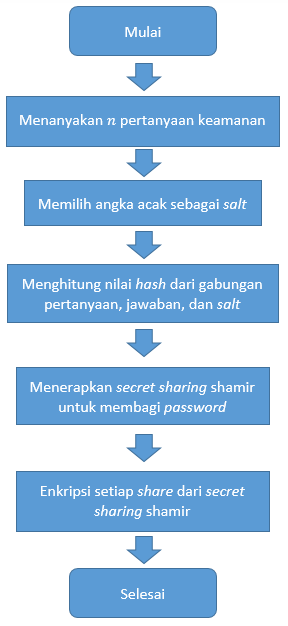
\includegraphics[scale=0.7]{Gambar/flowchart_share}}
	\caption{Proses Penyimpanan \textit{Password}}\label{fig:create_share}
\end{figure}

Secara umum, proses penyimpanan \textit{password} memiliki tahapan yang sama. Perbedaannya terdapat pada metode yang digunakan untuk masing-masing tahapan. Dalam penelitian ini, pembangunan \textit{share} menggunakan metode \textit{secret sharing} Shamir. Berikut penjelasan masing-masing tahapan:

\begin{itemize}
	\item Tahap Pembangunan \textit{Share} \\
	Pada tahap ini, dibutuhkan data-data masukan seperti $n$, $k$, dan $n$ \textit{password}. \textit{Password} diperoleh dari masukan pengguna. $n$ diperoleh dari banyak \textit{password} yang dimasukan pengguna. $k$ ditentukan dengan cara yang sudah dijelaskan pada Subbab \ref{subsec:pilihnk}.
	\item Tahap Pembuatan Digest \\
	Pada tahap ini, dibutuhkan data-data masukan juga seperti pertanyaan keamanan, jawaban dari pertanyaan keamanan, dan \textit{salt}. Pertanyaan keamanan dan jawaban dari pertanyaan keamanan diperoleh dari masukan pengguna. Sementara itu, \textit{salt} dipilih secara acak. Setelah itu, pertanyaan, jawaban, dan \textit{salt} akan dikonkatenasi menjadi sebuah \textit{string} yang akan dibuat \textit{digest}nya. Dalam tahap ini, pembuatan \textit{digest} akan menggunakan algoritma \textit{SHA}-512 (Subbab\ref{sec:SHA512}).
	\item Tahap Enkripsi \\
	Pada tahap ini, \textit{share} yang dihasilkan pada tahap pembangunan \textit{share} akan dienkripsi dengan menggunakan \textit{Data Encryption Standard} (Subbab \ref{sec:des}). \textit{Digest} yang dihasilkan pada tahap pembuatan \textit{digest} akan digunakan sebagai kunci proses enkripsi. Kemudian, \textit{ciphertext} dari \textit{share} hasil enkripsi akan disimpan.
\end{itemize}

\subsection{Proses Rekonstruksi \textit{Password}}

Pada bagian ini akan dijelaskan tahapan dari proses rekonstruksi \textit{password}. Flowchart dari proses rekonstruksi password ditunjukkan pada Gambar \ref{fig:flowchart_reconstruct_secret}.

%diagram
\begin{figure}[H]
	\centerline{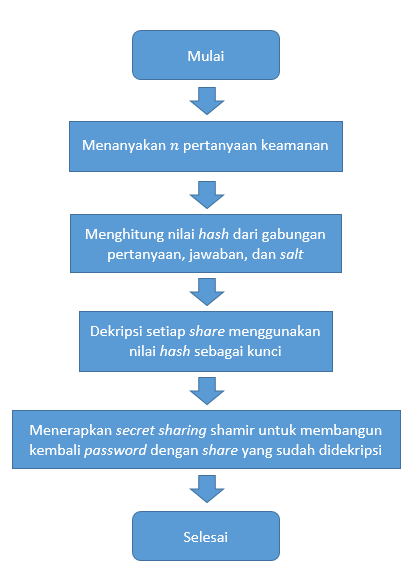
\includegraphics[scale=0.65]{Gambar/flowchart_reconstruct}}
	\caption{Proses Rekonstruksi \textit{Password}}\label{fig:flowchart_reconstruct_secret}
\end{figure}

Tahapan-tahapan ini pada proses yang ditunjukkan oleh Gambar \ref{fig:flowchart_reconstruct_secret} adalah tahapan untuk merekonstruksi \textit{password}. Tujuan dari proses rekonstruksi \textit{password} adalah mengembalikan password yang sudah disimpan. Berikut dijelaskan tahapan-tahapan dalam proses rekonstruksi \textit{password}:

\begin{itemize}
	\item Tahap Pembuatan \textit{Digest} \\
	Tahap pembuatan \textit{digest} ini sama dengan tahap pembuatan \textit{digest} dalam proses penyimpanan \textit{password}. Perbedaannya adalah pertanyaan keamanan dan nilai \textit{salt} diperoleh dari berkas teks yang disimpan. Sementara itu, jawaban dari pertanyaan keamanan tetap diperoleh dari masukan pengguna.
	\item Tahap Dekripsi \\
	Pada tahap ini, \textit{ciphertext} yang sudah disimpan akan didekripsi. Namun, sebelum proses dekripsi dilakukan, dibutuhkan beberapa data masukan \textit{digest} yang diperoleh dari tahap pembuatan \textit{digest}. Data masukan \textit{digest} digunakan sebagai kunci dalam proses dekripsi. Proses dekripsi pada tahap ini menggunakan \textit{Data Encryption Standard} (Subbab \ref{sec:des}).
	\item Tahap Rekonstruksi \textit{Share} \\
	Pada tahap ini, \textit{share} yang dihasilkan dari tahap dekripsi akan direkonstruksi untuk memperoleh \textit{password}. Tidak ada masukan pengguna dalam tahap ini. Metode rekonstruksi \textit{password} yang digunakan pada tahap ini adalah \textit{secret sharing} Shamir.
\end{itemize}

\section{Diagram}

Pada bagian ini akan dibuat diagram-diagram untuk perangkat lunak yang akan dibangun. Diagram-diagram ini dibuat berdasarkan analisis proses yang sudah dijelaskan pada Subbab \ref{sec:analisis}.

\subsection{Diagram \textit{Use Case}}

Perangkat lunak yang dibangun akan memiliki 2 fitur utama, yaitu menyimpan \textit{password} beserta pertanyaan keamanan yang sifatnya personal dan mengembalikan \textit{password}. Saat menyimpan \textit{password}, pengguna akan diminta untuk menambahkan pertanyaan keamanan yang sifatnya personal dan saat mengembalikan \textit{password}, pengguna akan diminta untuk menjawab pertanyaan keamanan yang sudah disimpan saat menyimpan \textit{password}. Gambar \ref{fig:use_case} menunjukkan diagram \textit{use case} dari perangkat lunak.

%diagram
\begin{figure}[H]
	\centerline{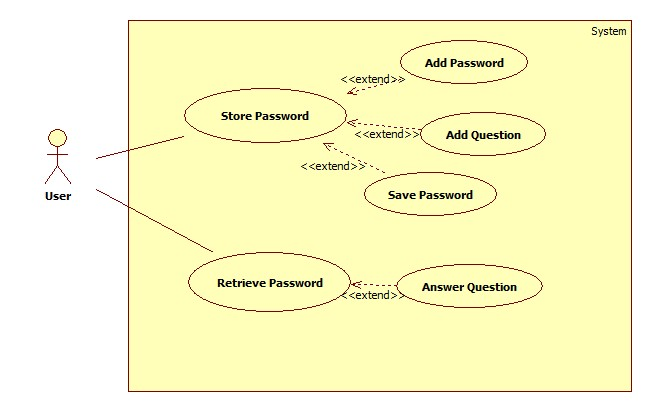
\includegraphics[scale=0.5]{Gambar/use_case}}
	\caption{Diagram \textit{use case} dari perangkat lunak}\label{fig:use_case}
\end{figure}

Adapun skenario-skenario yang pengguna dapat lakukan. Skenario untuk menyimpan \textit{password} ditunjukkan oleh Tabel \ref{table:scenario1}. Aktor dari skenario ini adalah pengguna dari sistem. Data masukan dari skenario ini adalah $n$ \textit{password} dan $n$ pertanyaan keamanan.

\begin{table}[H]
	\centering
	\caption{Skenario Menyimpan \textit{Password}} \label{table:scenario1}
	\begin{tabular}{|l|p{12cm}|}
		\hline
		\textbf{Nama} 					& Menyimpan \textit{Password} 																											\\ \hline
		\textbf{Aktor}					& Pengguna																																					\\ \hline
		\textbf{Deskripsi} 			& Pengguna menyimpan \textit{password} 																							\\ \hline
		\textbf{Kondisi Awal} 	& Aplikasi sudah dijalankan																													\\ \hline
		\textbf{Kondisi Akhir}	& \textit{share} sudah disimpan dalam berkas teks dalam bentuk \textit{ciphertext}	\\ \hline
		\textbf{Skenario Utama} & \begin{enumerate}[itemsep=0mm]\item Pengguna memasukkan \textit{password} dan pertanyaan keamanan \item \textit{Password} dan pertanyaan keamanan diterima oleh sistem\end{enumerate} \\ \hline
		\textbf{Eksepsi}				& Bila masukan tidak valid, sistem akan memberi peringatan \\ \hline
	\end{tabular}
\end{table}

Skenario untuk mengembalikan \textit{password} ditunjukkan oleh Tabel \ref{table:scenario2}. Aktor dari skenario ini adalah pengguna dari sistem. Data masukan dari skenario ini adalah $n$ jawab dari pertanyaan keamanan yang sudah dibuat.

\begin{table}[H]
	\centering
	\caption{Skenario Menyimpan \textit{Password}} \label{table:scenario1}
	\begin{tabular}{|l|p{12cm}|}
		\hline
		\textbf{Nama} 					& Mengembalikan \textit{Password} 																									\\ \hline
		\textbf{Aktor}					& Pengguna																																					\\ \hline
		\textbf{Deskripsi} 			& Pengguna mengembalikan \textit{password} 																					\\ \hline
		\textbf{Kondisi Awal} 	& Aplikasi sudah dijalankan	serta \textit{share}, pertanyaan keamanan, dan \textit{salt} sudah disimpan  \\ \hline
		\textbf{Kondisi Akhir}	& Sebanyak $n$ \textit{password} bisa dikembalikan																	\\ \hline
		\textbf{Skenario Utama} & \begin{enumerate}[itemsep=0mm]\item Pengguna menjawab setiap pertanyaan keamanan sebagai masukan \item Masukan diterima oleh sistem \item Sistem memberikan hasil pemrosesan berupa $n$ \textit{password}\end{enumerate} \\ \hline
		\textbf{Eksepsi}				& Bila masukan tidak valid, sistem akan memberi peringatan \\ \hline
	\end{tabular}
\end{table}

\subsection{Diagram Aktivitas}

Perangkat lunak yang dibangun memiliki 2 proses, yaitu menyimpan \textit{password} dan mengembalikan \textit{password}. Urutan aktivitas yang dilakukan perangkat lunak dalam proses menyimpan \textit{password} ditunjukkan pada diagram aktivitas \ref{fig:activity1}.

%diagram
\begin{figure}[H]
	\centerline{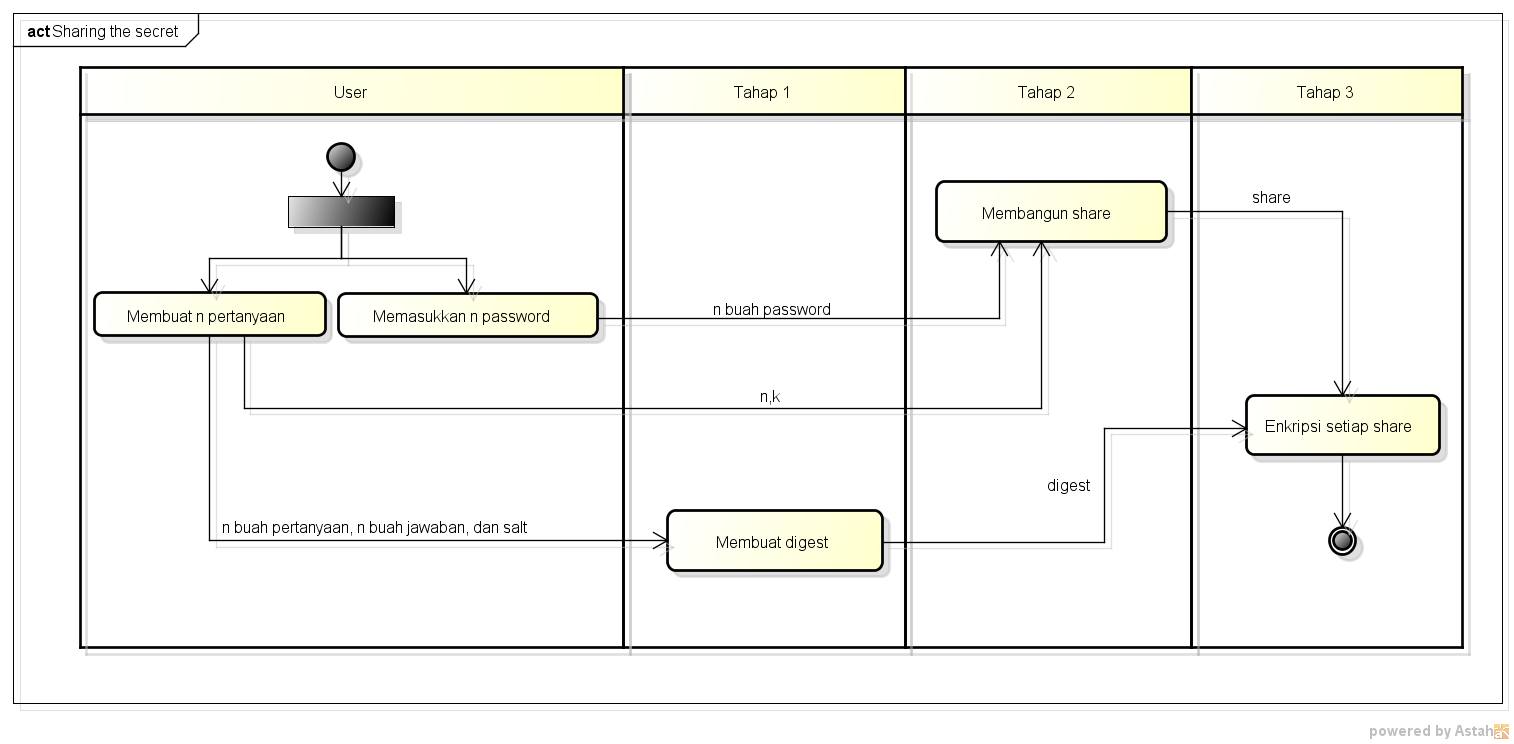
\includegraphics[scale=0.4]{Gambar/sharing-secret}}
	\caption{Diagram aktivitas untuk menyimpan \textit{password}}\label{fig:activity1}
\end{figure}

Dalam proses menyimpan \textit{password}, pengguna memasukkan $n$ \textit{password}. Kemudian, setelah memasukkan $n$ password, pengguna akan membuat $n$ pertanyaan keamanan dan jawaban masing-masing pertanyaan keamanan. Sistem akan menghitung $k$, yaitu minimal banyak pertanyaan yang harus dijawab benar oleh pengguna. Setelah itu, sistem akan memilih secara acak nilai \textit{salt}.

Setelah semua masukan yang dibutuhkan ada, sistem akan membuat \textit{digest} dari konkatenasi setiap pertanyaan keamanan, jawaban, dan nilai \textit{salt}. Sistem juga akan membangun \textit{share} dari masukan \textit{password}. Selanjutnya sistem akan mengenkripsi setiap \textit{share} dari masing-masing \textit{password} dan menggunakan \textit{digest} dari konkatenasi setiap pertanyaan keamanan, jawaban, dan nilai \textit{salt} sebagai kunci proses enkripsi. Setelah proses enkripsi, sistem akan menyimpan seluruh \textit{share} yang sudah dibangun, pertanyaan yang dibuat, $k$, dan nilai \textit{salt}.

Selanjutnya adalah proses mengembalikan \textit{password}. Gambar \ref{fig:activity2} menunjukkan diagram aktivitas untuk proses mengembalikan \textit{password}.

%diagram
\begin{figure}[H]
	\centerline{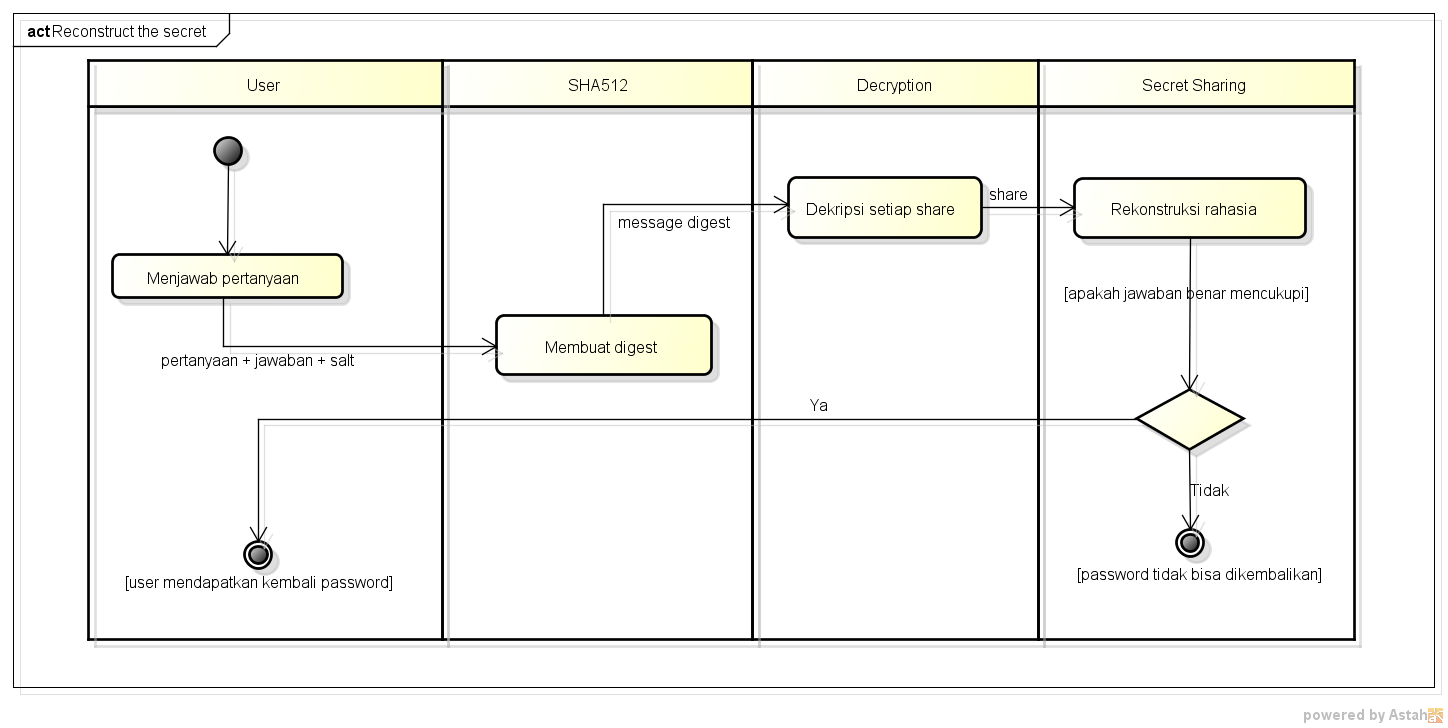
\includegraphics[scale=0.4]{Gambar/reconstruct-secret}}
	\caption{Diagram aktivitas untuk mengembalikan \textit{password}}\label{fig:activity2}
\end{figure}

Dalam proses untuk mengembalikan \textit{password}, pengguna akan diminta untuk menjawab $n$ pertanyaan keamanan yang disimpan saat proses penyimpanan \textit{password}. Sistem akan membuat digest dari konkatenasi setiap pertanyaan keamanan, jawaban pertanyaan keamanan dari masukan pengguna, dan nilai \textit{salt} yang disimpan.

Selanjutnya, sistem akan melakukan proses dekripsi setiap \textit{share} yang sudah disimpan dan menggunakan \textit{digest} sebagai kunci proses dekripsi. Setelah semua \textit{share} didekripsi, sistem akan merekonstruksi \textit{password} dengan \textit{share} dan nilai $k$ yang disimpan sebagai masukan. Jika proses rekonstruksi berhasil, maka pengguna dapat mengembalikan \textit{password}. Sebaliknya, jika proses rekonstruksi gagal, maka \textit{password} tidak bisa dikembalikan.

\subsection{Diagram Kelas}

Pada bagian ini akan dibuat diagram kelas dari perangkat lunak yang akan dibangun. Kelas-kelas ini merupakan rancangan kelas yang dibutuhkan untuk membangun perangkat lunak dan dibuat berdasarkan proses-proses yang sudah dijelaskan pada Subbab \ref{sec:analisis}. Rancangan diagram kelas dari perangkat lunak yang dibangun ditunjukkan oleg Gambar \ref{fig:diagramkelasdummy}.

%diagram
\begin{figure}[H]
	\centerline{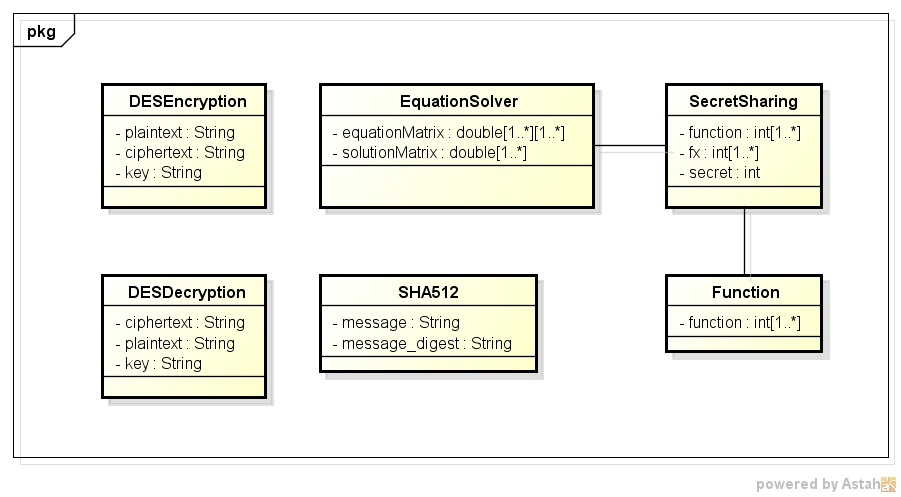
\includegraphics[scale=0.6]{Gambar/engine-class-diagram}}
	\caption{Rancangan Diagram Kelas}\label{fig:diagramkelasdummy}
\end{figure}

Adapun diagram kelas yang ditunjukkan oleh Gambar \ref{fig:diagramkelasdummy} terdiri dari:

\begin{enumerate}
	\item Kelas \textit{DESEncryption} \\
	Kelas \textit{DESEncryption} merupakan kelas yang berperan untuk melakukan proses enkripsi setiap \textit{share}. Kelas ini mengimplementasikan algoritma \textit{Data Encryption Standard} untuk proses enkripsinya.
	\item Kelas \textit{DESDecryption} \\
	Kelas \textit{DESDecryption} merupakan kelas yang berperan untuk melakukan proses dekripsi setiap \textit{share}. Kelas ini mengimplementasikan algoritma \textit{Data Encryption Standard} untuk proses dekripsinya.
	\item Kelas \textit{SHA}512 \\
	Kelas ini berperan untuk membuat \textit{digest} dari konkatenasi masing-masing pertanyaan, jawaban, dan \textit{salt}. Kelas ini mengimplementasikan algoritma \textit{SHA}-512 untuk proses pembuatan \textit{digest}.
	\item Kelas \textit{Secret Sharing} \\
	Kelas ini berperan dalam pembangunan \textit{share}. Kelas ini menggunakan metode \textit{secret sharing} Shamir untuk proses pembangunan \textit{share}.
	\item Kelas Writer \\
	Kelas yang berperan untuk menyimpan setiap keluaran ke dalam berkas teks.
	\item Kelas Reader \\
	Kelas yang berperan untuk membaca berkas teks dan hasil bacaannya akan digunakan sebagai masukan.
\end{enumerate}